\documentclass[12pt,floatfix,showpacs]{revtex4-1}

\usepackage{amssymb,amsmath,amsfonts}
\usepackage{graphicx}

\newcommand{\eg}{\emph{e.g., }}
\newcommand{\ie}{\emph{i.e., }}
\newcommand{\etal}{\emph{et al.}}

% remove these for final publication 
\usepackage{color} 
\newcommand{\note}[1]{\textcolor{red}{#1}}
\newcommand{\gnote}[1]{\marginpar{\textcolor{red}{\scriptsize{#1}}}}

\graphicspath{{./graphics/}{./pdfgraphics/}}  % remove pdfgraphics path for final publication!

\begin{document}

\title{Stability and Edge-Localized Mode Characterization in I-Mode Pedestals}

\author{JR Walk}
\email[]{jrwalk@psfc.mit.edu}
\affiliation{MIT Plasma Science and Fusion Center}

\author{JW Hughes}
\affiliation{MIT Plasma Science and Fusion Center}

\author{PB Snyder}
\affiliation{General Atomics}

\author{AE Hubbard}
\affiliation{MIT Plasma Science and Fusion Center}

\author{B LaBombard}
\affiliation{MIT Plasma Science and Fusion Center}

\author{DF Brunner}
\affiliation{MIT Plasma Science and Fusion Center}

\author{JL Terry}
\affiliation{MIT Plasma Science and Fusion Center}

\author{DG Whyte}
\affiliation{MIT Plasma Science and Fusion Center}

\author{AE White}
\affiliation{MIT Plasma Science and Fusion Center}

\author{E Edlund}
\affiliation{Princeton Plasma Physics Laboratory}

\date{\today}

\begin{abstract}
I-mode is a novel high-confinement tokamak regime characterized by H-mode-like enhanced energy confinement and the formation of a strong temperature pedestal, without the accompanying density pedestal or enhanced particle confinement, maintaining an L-mode-like density profile.  I-mode exhibits a number of desirable properties for a reactor regime, including a lack of strong degradation of energy confinement with heating power and apparent naturally-occurring suppression of large ELMs, avoiding the need for externally-applied ELM suppression.  However, under certain conditions (particularly, reduced toroidal field) small, intermittent ELM-like events are seen, although these cases are modeled to be stable to the peeling-ballooning MHD instability associated with the ELM trigger, as is typical of I-mode pedestals.  We examine these events in detail to better characterize the edge stability behavior in I-mode.  The majority of observed ELM candidates are observed to be synchronized with the sawtooth heat pulse reaching the pedestal, which measurably perturbs the temperature pedestal.  However, this perturbation appears to be insufficient to reach the peeling-ballooning stability boundary; moreover, the ELM candidate does not include a ``crash'' in the pedestal temperature or stored energy.  \note{precursor fluctuations?  include Ahmed?  Ref divertor heat flux measurements?}  In short, these events do not appear to be true instability-driven ELMs, but rather are benign $H_\alpha$ spikes driven by the sawtooth heat pulse.  A minority of the ELM candidates in I-mode do include the characteristic temperature crash associated with an ELM, and are not necessarily sawtooth-triggered -- however, these events are isolated, and the stationary pedestal structure in these I-modes is also modeled to be stable to the ELM trigger, indicating that transient events in the pedestal drive these ELMs, rather than an inherent instability of the pedestal.
\end{abstract}

\pacs{52.55.Fa, 52.55.Tn, 52.35.Py, 52.25.Fi, 52.40.Hf}

\maketitle

%%%%%%%%%%%%%%%%%%%%%%%%%%%%%%%%%%%%%%%%%%%%%%%%%%%%%%

\section{Introduction}\label{sec:intro}

The development of tokamak magnetic-confinement fusion into a viable \& economical form of power generation faces two overarching (and seemingly contradictory) requirements.  
First, a high level of energy confinement is necessary for net energy production with the desired level of self-heating of the plasma by fusion products.  
At the same time, sufficient particle transport is needed to avoid the deleterious effects of accumulated impurities (both helium ``fusion ash'' and higher-$Z$ impurities from the erosion of plasma-facing components) due to fuel dilution and radiative losses.  
This has been achieved in a number of operating regimes, collectively termed ``high-confinement'' or H-modes \cite{Wagner1982}.  

H-modes are characterized by a steep gradient region at the plasma edge in density, temperature, and pressure, termed the \emph{pedestal}, the height of which is strongly correlated with global fusion performance \cite{Kinsey2011}.  
These strong gradients have been shown to drive edge MHD instabilities \cite{Huysmans2005,Maget2013,Snyder2002} resulting in an Edge-Localized Mode (ELM), an explosive perturbation to the pedestal expelling energy and particles into the plasma exhaust \cite{Zohm1996}.  
On existing experiments, ELMs drive sufficient particle transport to allow stationary operation with acceptable radiative losses \cite{Keilhacker1984}; as ELMy H-modes are robust and straightforward to achieve, this regime is considered the baseline for ITER operation \cite{ITER1999,Shimada2007}.  
However, on ITER-scale devices ELMs drive transient heat loads to the divertor, leading to unacceptable levels of erosion and damage to plasma-facing components \cite{Loarte2003,Federici2003}.
This introduces an additional requirement for tokamak fusion reactor concepts -- the avoidance, suppression, or mitigation of large ELMs, either via externally-applied engineering solutions (pellet pacing \cite{Baylor2013,Lang2014} or resonant magnetic perturbations \cite{Evans2004,Evans2006}), or via alternate high-confinement regimes which regulate the pedestal below the ELM limit (\eg the Enhanced $D_\alpha$ (EDA) H-mode \cite{Greenwald1999,Hubbard2001} or the QH-mode \cite{Burrell2002,Suttrop2005}).

\begin{figure}[p] % shift to ht placement!
 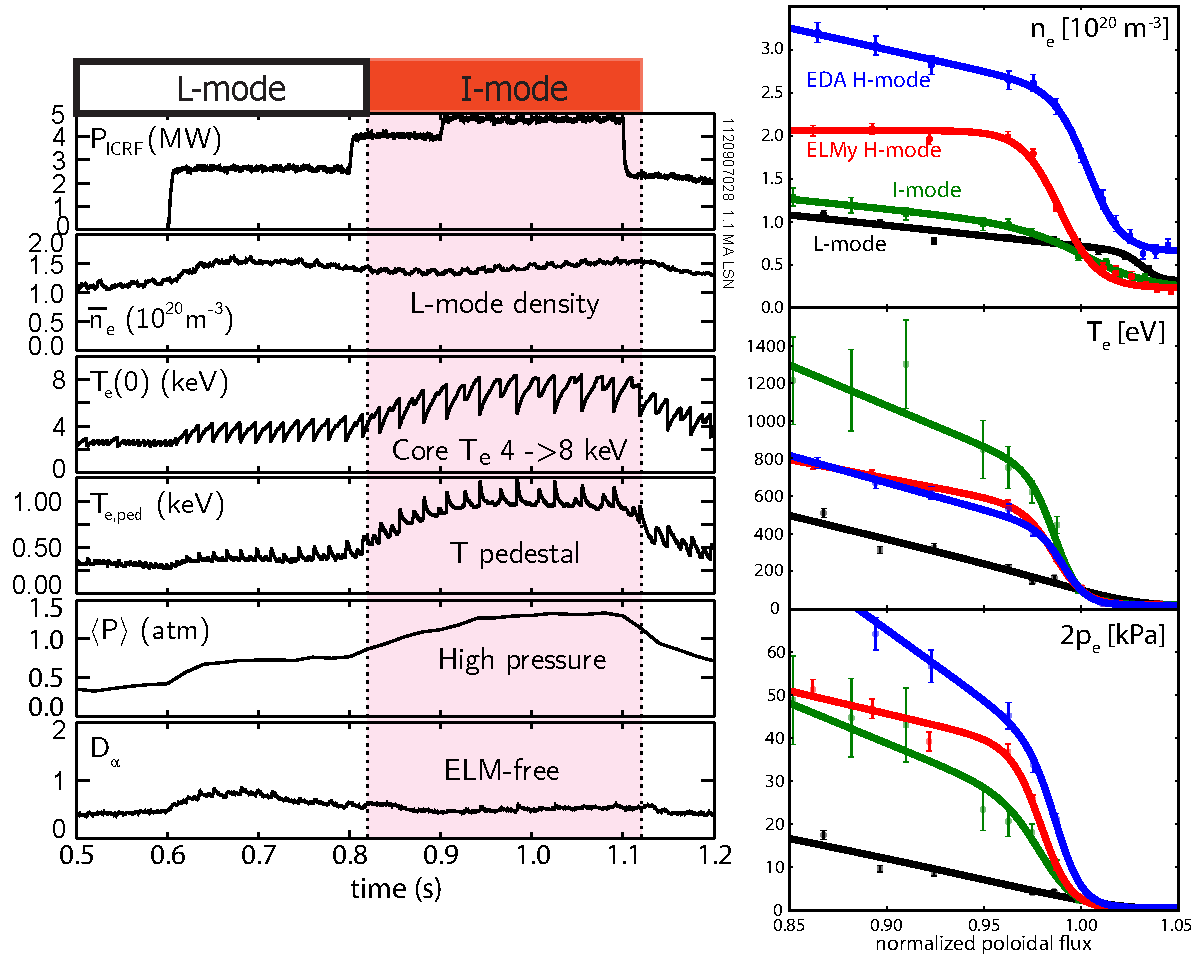
\includegraphics[width=\textwidth]{trace_imode.pdf}
 \caption{(left) characteristic time traces for an I-mode.  After the L-I transition, the core and edge temperature rise over several sawtooth cycles (visible in the oscillations in $T_e(0)$ and $T_{e,ped}$) before reaching a steady level; global pressure and confinement rise accordingly.  However, the density remains unchanged from the L-mode level.  No ELMs are exhibited on the $D_\alpha$ trace.  (right) pedestal profiles for L-, I-, and H-modes.  The I-mode (green) retains a density profile similar to L-mode (black), unlike the ELMy (red) and EDA (blue) H-modes, which form a strong density pedestal.  However, the I-mode forms a higher temperature pedestal than either H-mode, resulting in comparable pedestal pressures to H-mode while retaining L-mode particle transport.}
 \label{fig:imode_trace}
\end{figure}

The I-mode \cite{Whyte2010,Hubbard2011,Walk2014,Walk2014b}, pioneered on the Alcator C-Mod tokamak \cite{Hutchinson1994}, is one such alternate regime for high-performance operation.  
I-mode is notably unique among high-performance regimes in that it apparently decouples energy and particle transport, attaining the desired H-mode-like energy confinement while retaining L-mode particle transport, naturally achieving the desired low level of impurity confinement \cite{Howard2011}.\note{other cites?}  
This manifests in the edge by the formation of a strong temperature pedestal without the accompanying density pedestal found in conventional H-modes (see Figure~\ref{fig:imode_trace}).  
I-mode also exhibits minimal degradation of energy confinement with heating power \cite{Whyte2010,Dominguez2012,Walk2014b}, in contrast to the degradation of confinement found in ELMy H-mode (roughly $\tau_E \sim P^{-0.7}$ from multi-machine analyses \cite{Christiansen1992,ITER1999}), a potentially highly favorable result for a reactor regime.

The I-mode appears to generally lack large ELMs, obviating the need for externally-applied engineering solutions; however, as has been previously reported \cite{Whyte2010,Walk2014,Walk2014b}, under certain conditions (particularly at reduced toroidal field) small, intermittent ELMs have been observed.
In this paper, we examine these intermittent events through computational modeling of the instabilities associated with the ELM trigger and experimental observations of edge behavior in I-mode.  \note{sort out outline}

\section{I-Mode Access \& Experimental Setup}\label{sec:setup}

The I-mode experiments presented here were carried out on the Alcator C-Mod tokamak \cite{Hutchinson1994}, a compact, high-field device with major radius $R \sim 0.67 \;\mbox{m}$, minor radius $a \sim 0.22 \;\mbox{m}$, and toroidal field up to $B_T \le 8.1 \;\mbox{T}$.  
C-Mod operates with entirely high-$Z$ metal plasma-facing components, and reaches comparable heat flux to the divertor to that expected for ITER \cite{Loarte2007,Terry2007,LaBombard2011}, making it a uniquely-suited test bed for SOL and divertor experiments in support of ITER\gnote{too much?}.  
High-performance operation is commonly assisted by boronization treatment of plasma-facing materials -- however, due to the low impurity confinement in I-mode a recent boronization is not critical for these experiments.  
Alcator C-Mod plasmas are purely RF heated with up to $5.5 \;\mbox{MW}$ of ion-cyclotron heating power.

I-mode operation is most attainable in the so-called ``unfavorable'' drift configuration -- that is, with the ion $\nabla B$ drift directed away from the primary X-point \cite{Whyte2010}.  
This elevates the H-mode power threshold \cite{Hubbard2007}, widening the power range between L- and H-mode available for I-mode operation.  
This drift configuration both in upper-single-null (USN) shapes, and in the more typical lower-single-null (LSN) shapes with the toroidal field reversed (plasma current direction is reversed as well to preserve field helicity)\gnote{clarify?}.  
Brief I-mode periods have also been observed in the favorable drift configuration, but these transitioned quickly to H-mode and are not considered for the purposes of this paper.

Provided the unfavorable drift condition is met, I-mode operation is quite robustly accessible on Alcator C-mod, with steady I-modes attained in a number of shapes and edge current profiles -- notably, I-mode operates naturally near the values for edge safety factor and collisionality targeted for ITER.  
The data presented here were taken in dedicated I-mode experiments focusing on reversed-field LSN operation to optimize the plasma for pedestal and edge diagnostic coverage and high-quality pedestal profiles for modeling purposes.  
In a subset of these experiments, small, intermittent ELMs were observed -- while the conditions leading to these events are not well-understood, they are particularly found in operation at reduced field ($B_T \sim 4.6 \;\mbox{T}$).  
These results are the focus of this paper, with broader results from the pedestal study reported by Walk \emph{et al.} \cite{Walk2014}.\gnote{get formatting right}

\section{I-Mode Pedestal Stability \& Modeling}\label{sec:model}

\subsection{Pedestal Modeling}\label{subsec:ped_mod}

Large, uncontrolled ELMs in ITER operation are expected to drive unacceptable levels of pulsed heat loading and erosion damage to wall and divertor surfaces \cite{Loarte2003,Federici2003} -- as such, avoiding, mitigating, or suppressing large ELMs is a major focus in research on high-performance regimes.  
Confidence in plans for high-performance operation on ITER- and reactor-scale devices without large ELMs requires a predictive, first-principles understanding of the pedestal structure and stability at the ELM limit.  
Recent cooperative efforts among theory, modeling, and experiment \cite{Groebner2013} has resulted in such a model, termed EPED (not an acronym) \cite{Snyder2009,Snyder2011}.  
The EPED model combines constraints from stability against peeling-ballooning MHD modes driven by the steep gradients in the pedestal \note {blah blah blah describe modeling gist}

\subsection{I-Mode Stability}\label{subsec:imode_mod}

\begin{figure}[ht]
 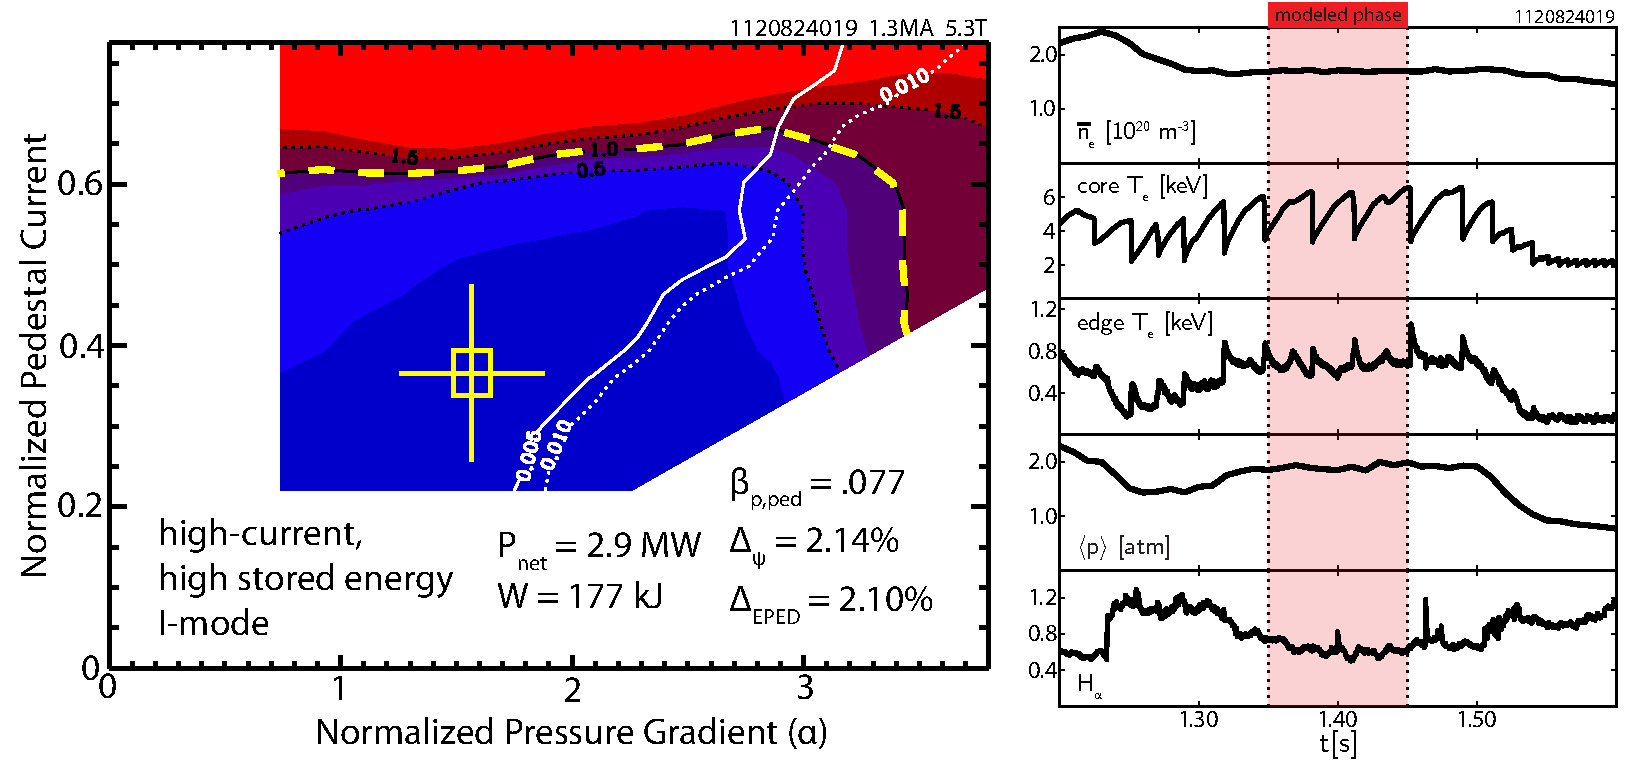
\includegraphics[width=\textwidth]{pdfgraphics/1120824019_ELITE_stitch_v2.pdf}
 \caption{MHD stability contour for high-current ($1.3 \;\mbox{MA}$), high-performance I-mode generated by the ELITE code.  The experimental measurement (with uncertainties) is shown by the crosshair, with the stability boundary (accounting for diamagnetic stabilization of the MHD mode) shown by the yellow dashed line.  Experimentally-measured parameters for the modeled phase are shown at right.  The white contours indicate calculations of the infinite-$n$ ballooning stability calculated by BALOO, used as a surrogate for the onset of KBM turbulence.  Due to the local nature of the infinite-n constraint, BALOO calculates the width in flux space that is locally ballooning-critical.  When this reaches half of the pedestal width, the KBM is assumed to be triggered. This case is near the KBM-predicted pedestal width $\Delta_{EPED}$, but is nevertheless modeled to be KBM-stable (for $\Delta_\psi \sim 0.02$, the half-width threshold is the white dotted contour labeled $0.01$.}
 \label{fig:elite_1120824019}
\end{figure}

An ELITE calculation for the I-mode pedestal, with BALOO calculations of the KBM threshold, is shown in Figure~\ref{fig:elite_1120824019}, along with parameters (line-averaged density, core and edge $T_e$, global average pressure, and $H_\alpha$ emission).  
The I-mode pedestal parameters, indicated with uncertainties by the yellow crosshair, are far from both the peeling and ballooning stability boundaries (indicated by the yellow dashed line).  
This is consistent with the observed lack of large ELMs in I-mode, even in high-performance cases (both in the normalized sense, with $H_{98} = 1.02$ and $\langle \beta_N \rangle = 1.0$, and absolute terms, with $W_{MHD} = 177 \;\mbox{kJ}$ for the case in Figure~\ref{fig:elite_1120824019}, compared to $W \sim 100-120\;\mbox{kJ}$ for ELMy H-mode and $W \sim 150-190\;\mbox{kJ}$ for EDA H-mode typical on C-Mod).

\begin{figure}[ht]
 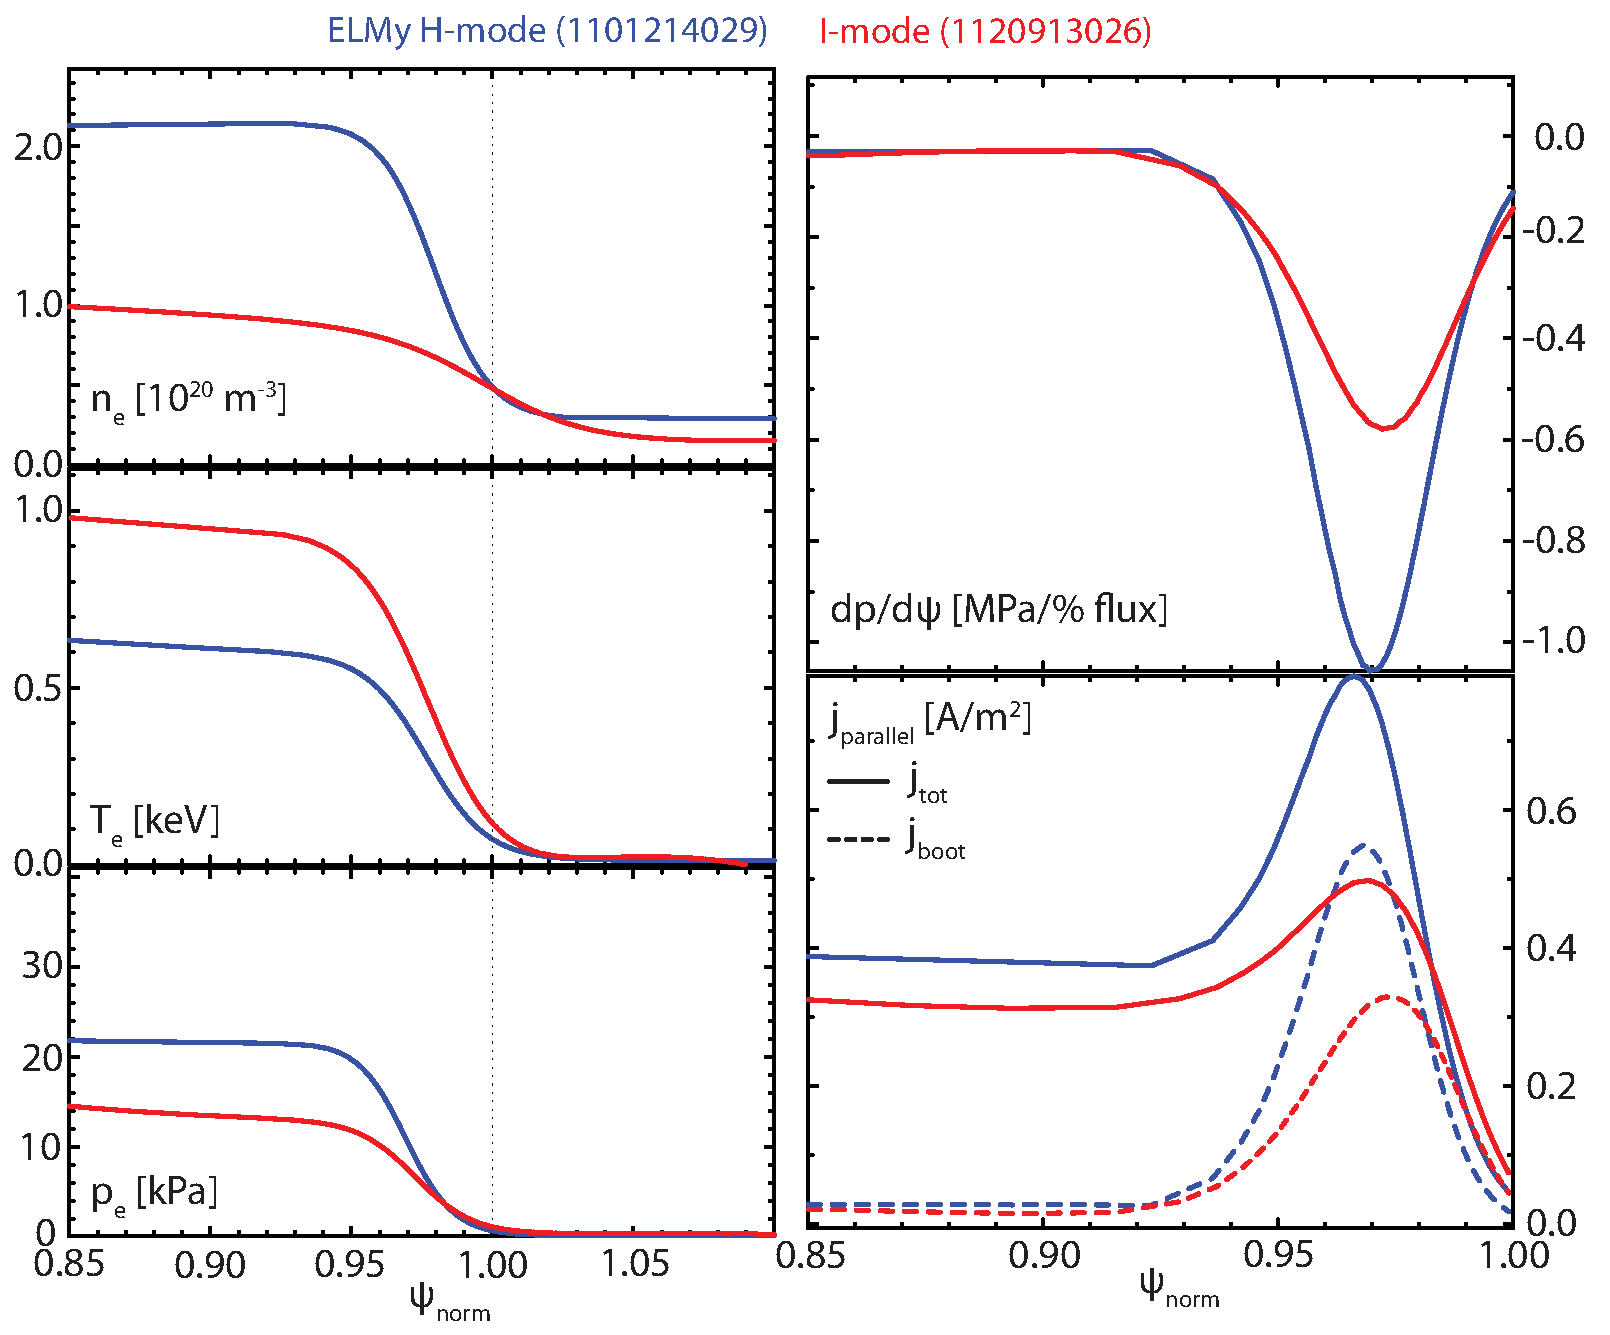
\includegraphics[width=0.75\textwidth]{pdfgraphics/prof_elmy_imode.pdf}
 \caption{Pedestal profiles in I-mode and ELMy H-mode. Due to the steep density gradient in the pedestal, the H-mode exhibits significant pressure gradient and edge current density, which drive the peeling-ballooning MHD instability associated with the ELM trigger. Despite this, the high edge temperature in I-mode allows it to reach an appreciable pedestal pressure.}
 \label{fig:prof_elmy_imode}
\end{figure}

The calculated MHD stability is intuitively understood from the I-mode pedestal profile -- while the I-mode pedestal reaches comparable pressure to H-mode, the pressure is due largely to the strong temperature pedestal, with a relaxed density profile and broader pedestal than H-modes at comparable $\beta_{p,ped}$.  
This reduces the total pressure gradient (and thus the ballooning MHD drive), as well as the local bootstrap current density (set largely by the density gradient), thus reducing the peeling MHD drive as well.  A comparison of the pedestal profiles, with pressure gradient and edge current density, between I-mode and ELMy H-mode is shown in Figure~\ref{fig:prof_elmy_imode}.  
\note{move earlier, rework intro paragraph of section to be more general about peeling-ballooning stability, rather than ELITE specifically}

\subsection{Intermittent ELMs in I-Mode}\label{subsec:elms}

While I-mode is typically observed to be naturally free of large, damaging ELMs (consistent with the pedestal profile characteristics and modeled stability, shown in subsection~\ref{subsec:imode_ped_mod}), on occasion, small, intermittent events featuring the characteristic $H_\alpha$ spikes associated with ELMs have been observed in I-mode \cite{Whyte2010,Walk2014}.  
The conditions necessary for these events to arise are unclear, although they are most commonly observed at reduced plasma current and toroidal field.  
These events are small ($<1\%$ perturbation to the stored energy) and are sporadic, rather than occurring in a regular cycle as expected for conventional type-I ELMs.  
Moreover, I-mode cases exhibiting these events are modeled to be strongly stable against both peeling-ballooning MHD modes and the KBM turbulence trigger (see Figure~\ref{fig:elite_1120913026}).

\begin{figure}[ht]
 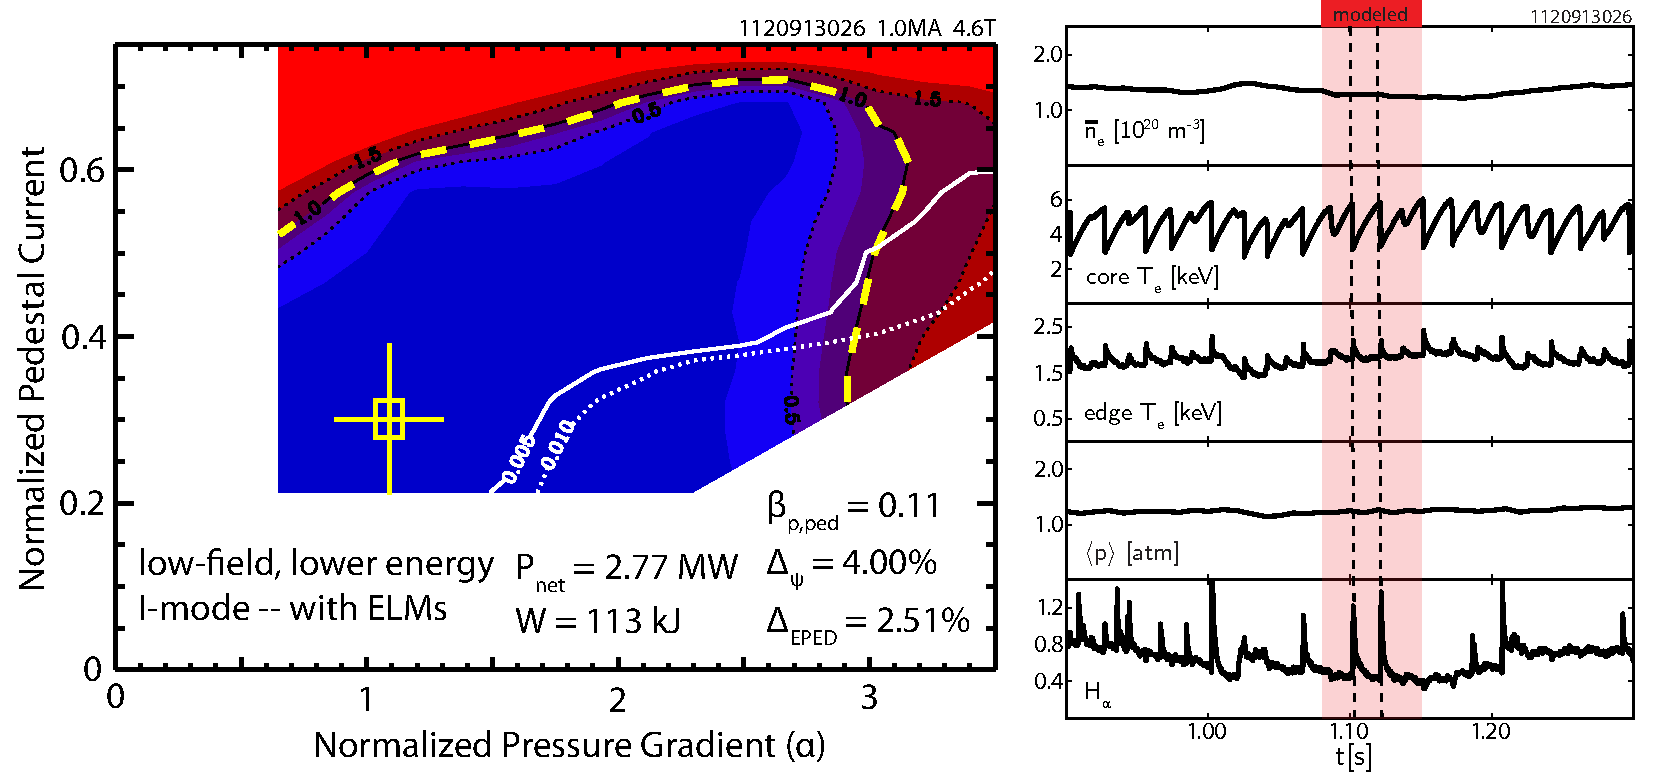
\includegraphics[width=\textwidth]{pdfgraphics/1120913026_ELITE_stitch_v3.pdf}
 \caption{Calculated MHD stability and KBM threshold characteristics of a low-field ($4.6\;\mbox{T}$) I-mode exhibiting small, intermittent ELM-like events, with experimental traces of the modeled phase at right.  Despite exhibiting ELM characteristics in the $H_\alpha$ trace, apparently triggered by the sawtooth heat pulse reaching the edge (visible on the edge ECE $T_e$ trace), the pedestal is modeled to be stable against the ELM trigger.}
 \label{fig:elite_1120913026}
\end{figure}

I-modes featuring these events comprise a minority of the studied cases -- out of the high-resolution pedestal database of 72 time windows (52 unique shots), 12 time windows (10 unique shots) exhibited the characteristic $H_\alpha$ spikes.
To better characterize these events, we consider the basic requirements of an ELM observation: the explosive perturbation is characterized by (1) a spike in $H_\alpha$ light associated with the burst in edge ionization, (2) a driving instability in the pedestal, (3) a crash in the pedestal temperature and pressure and associated spike in heat flux to the divertor.  
Identification of ELMs in I-mode is based on the observation of $H_\alpha$ spikes -- we now consider the other observations \note{reword}

\section{Sawtooth-Triggered Events}\label{sec:sawtooth}

The stationary pedestal profile in I-mode is seen to be stable against the peeling-ballooning MHD instability, as well as the limiting kinetic-ballooning turbulence, traditionally associated with the ELM trigger, even in cases with apparent ELM events.
However, I-modes on C-Mod typically present substantial sawtooth activity \note{cite? Hubbard, Whyte?}, which drives a regular heat pulse to the edge of the plasma.
In the majority \note{check number} of I-mode cases featuring observed ELMs, the ELM events are synchronized with the sawtooth heat pulse reaching the edge based on timing from fast ECE $T_e$ measurements in the pedestal, suggesting a trigger.
The impact of this heat pulse on the pedestal structure is shown in Figure~\ref{fig:prof_stbin}: while the heat pulse drives negligible perturbation to the density profile, it does significantly modify the edge temperature profile (data masked to the first 25\% of the sawtooth cycle are shown in red).

\begin{figure}[htp]
 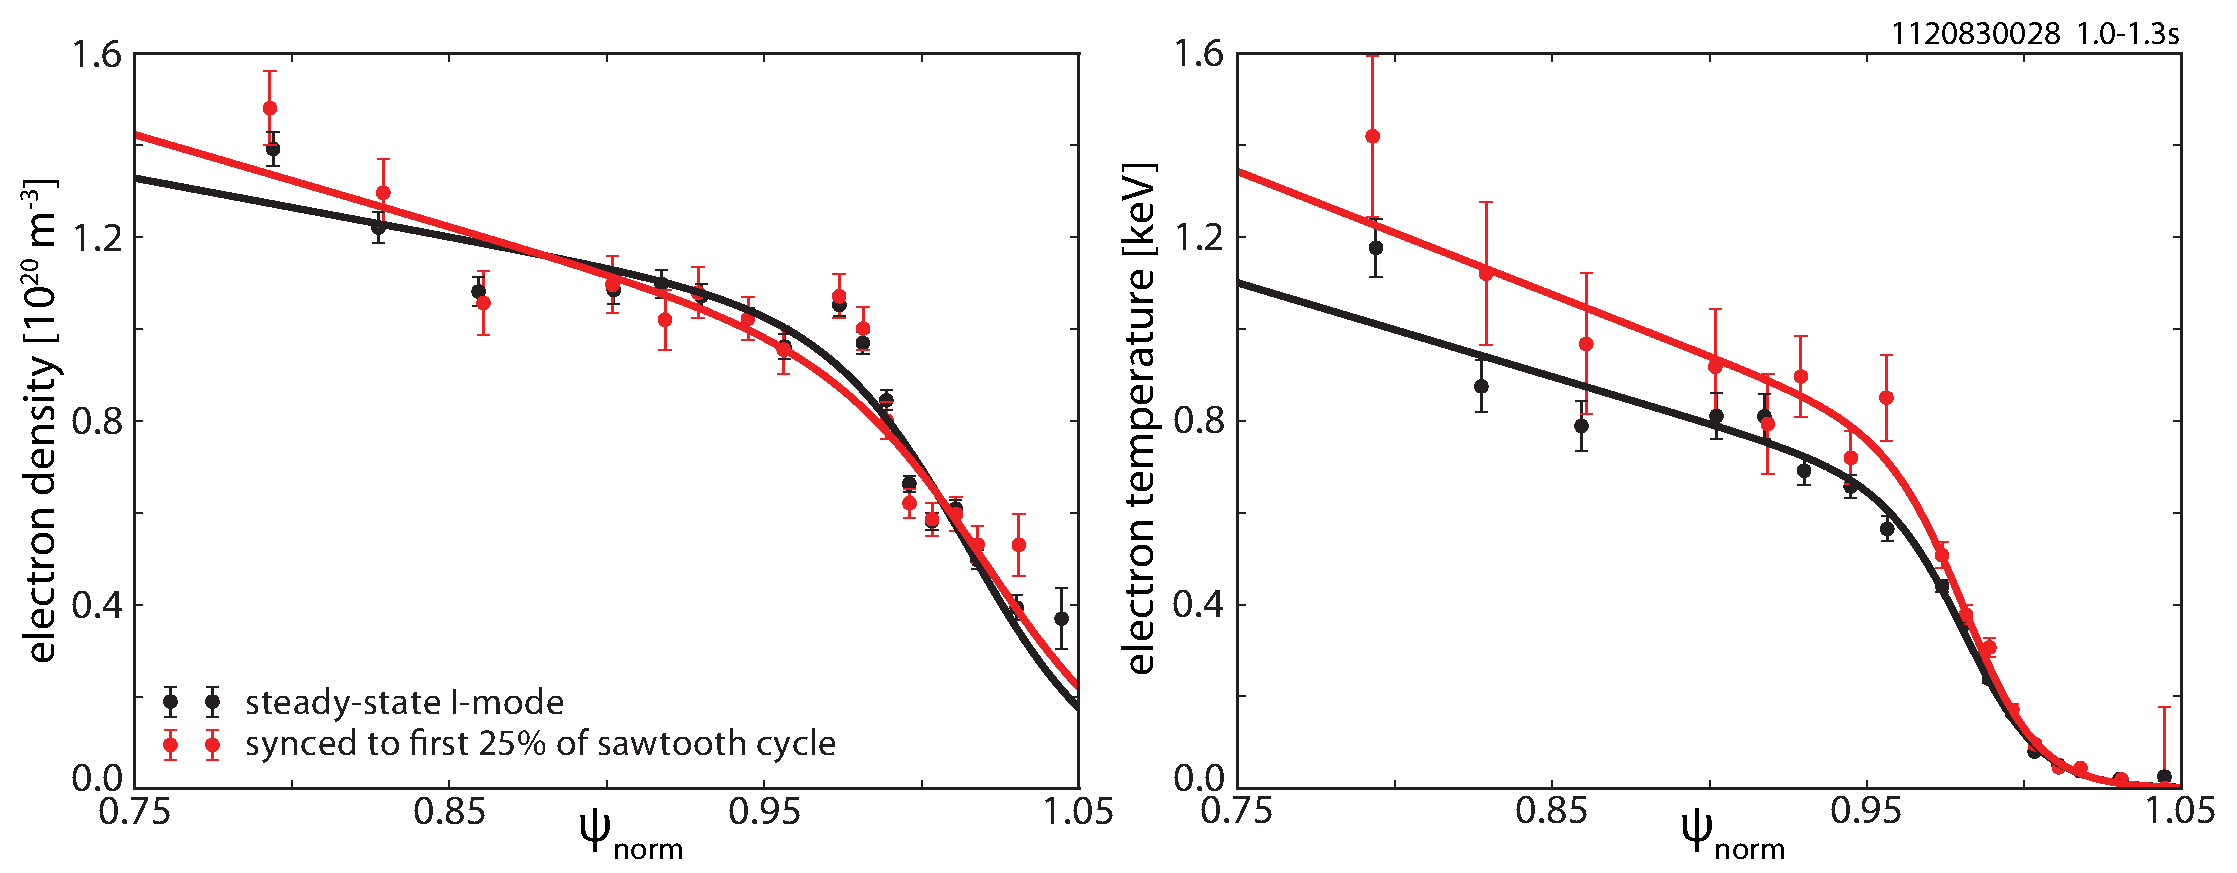
\includegraphics[width=\textwidth]{pdfgraphics/1120830028_prof_stbin.pdf}
 \caption{Sawtooth perturbation to the pedestal in I-mode, generated by masking profile data to the first 25\% of the sawtooth cycle.  The sawtooth heat pulse drives negligible perturbation to the density profile, but supplies a significant transient increase to the pedestal temperature.}
 \label{fig:prof_stbin}
\end{figure}

Calculations in ELITE and BALOO are shown in Figure~\ref{fig:1120830028_stbin_elite}.


\begin{figure}[htp]
 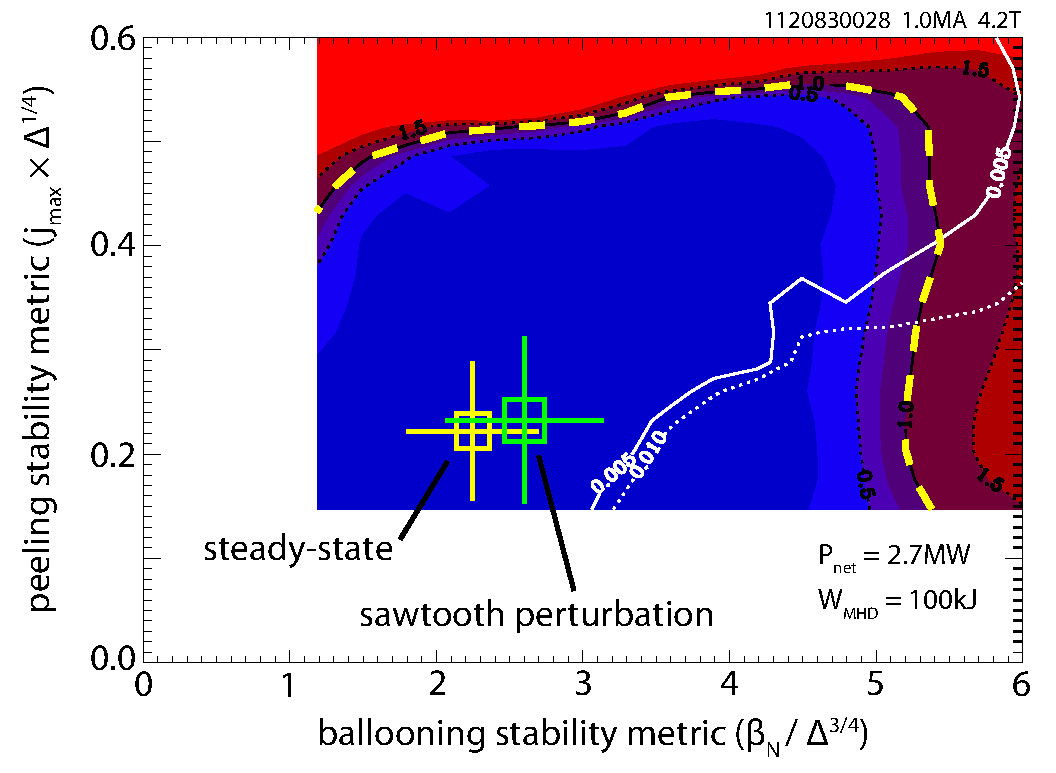
\includegraphics[width=\textwidth]{pdfgraphics/1120830028_stbin_elite.pdf}
 \caption{Peeling-ballooning MHD stability calculated by ELITE and KBM thresholds calculated by BALOO for an I-mode case, comparing the time-averaged data against pedestal profiles prepared with data masked to the first 25\% of the sawtooth cycle following a heat pulse reaching the edge.  Note that, to directly compare two separately-calculated equilibria, we replace the $\alpha_{MHD}$ and $j_\parallel$ axes with stability metrics arising from peeling and ballooning MHD.  While the sawtooth heat pulse does measurably perturb the pedestal in stability space, it is insufficient to reach either the peeling-ballooning or KBM threshold.}
 \label{fig:1120830028_stbin_elite}
\end{figure}

%%%%%%%%%%%%%%%%%%%%%%%%%%%%%%%%%%%%%%%%%%%%%%%%%%%%%%

\begin{acknowledgments}
 Experimental work on Alcator C-Mod is supported by US DOE agreement DE-FC02-99ER54512. Theory work at General Atomics is supported by US DOE agreement DE-FG02-99ER54309.  The authors also wish to acknowledge the efforts of the Alcator C-Mod team for supporting the experiments reported here.
\end{acknowledgments}

% remove \bibliography call, paste in bbl file
% actually, peerx-press says they accept bib files now!
% construct proper bib file once citations are all put together
\bibliographystyle{aipnum4-1}
\bibliography{jrwalk_references}

\end{document}